\section{11200 - Sapitaur's labyrinth}
\textbf{Problema:} 
Dada una grilla de paredes diagonales, determinar cu\'antos caminos hay desde
el borde superior de la grilla hasta el borde inferior.

\subsection{Resoluci\'on}

La entrada es una matriz de $n \times m$, que en la
posici\'on $(i,j)$ indica si la pared es una diagonal
ascendente (\texttt{/}) o descendente (\texttt{$\backslash$}).
Consideramos el grafo impl\'icito asociado a esta matriz.
El grafo en cuesti\'on tiene $(n + 1) \times m$ nodos, uno
por cada segmento horizontal de la grilla. Dos nodos
son adyacentes si, y solo si, est\'an en celdas contiguas y se puede
llegar de uno al otro sin cruzar una pared (y sin salir
de la grilla).

\begin{figure}[H]
\centering
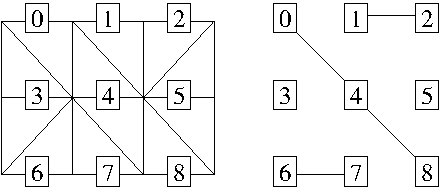
\includegraphics[scale=0.65]{./figuras/laberinto.pdf}
\caption{Grilla con paredes diagonales y el grafo asociado a esta grilla}
\label{fig:laberinto}
\end{figure}

El problema que se quiere resolver es entonces determinar la
cantidad de caminos
simples que empiezan en alguno de los nodos de la
primera fila ($0, 1, ..., m - 1$) y
terminan en alguno de los nodos de la \'ultima fila
($n m, n m + 1, ..., n m + m - 1$).

Los grafos asociados a este tipo de matrices cumplen las siguientes propiedades:

\begin{itemize}
\item Cada nodo tiene grado a lo sumo 2. Esto
es porque un segmento horizontal de la grilla puede
tener a lo sumo un vecino por la celda superior
(como el $0$ respecto del $4$ o la pareja $6$--$7$ en
la Fig.~\ref{fig:laberinto})
y a lo sumo un vecino por la celda inferior (como el $8$ respecto del $4$ o la pareja $1$--$2$). Notar que esto es cierto porque en
{\em todas} las celdas hay una pared.

\item Los nodos de la primera fila y los de la \'ultima
fila tienen grado a lo sumo 1. Los nodos de la primera fila no pueden
tener un vecino por la fila superior, y algo an\'alogo ocurre para los de la \'ultima.

\item Si bien el grafo puede tener ciclos,
no puede haber ciclos alcanzables desde los
nodos de la primera fila. M\'as a\'un, desde
los nodos de la primera fila s\'olo puede
construirse un \'unico camino simple maximal.
Por inducci\'on en la longitud del camino, es
f\'acil ver que todo camino simple
que empiece en un nodo $v_1$ de la primera fila
es o bien $v_1$ (si $v_1$ tiene grado 0)
o bien de la forma
$v_1, ..., v_k$ donde $v_1$ tiene grado 1,
$v_2, ..., v_{k-1}$ tienen grado 2
y $v_k$ tiene grado 1 \'o 2.
Uno de los vecinos de $v_k$ es $v_{k-1}$.
Si $v_k$ tiene grado 1, no tiene m\'as vecinos,
y por lo tanto este es
el \'unico camino simple maximal que se
puede construir a partir de $v_1$.
Si $v_k$ tiene grado 2, tiene un segundo vecino $v_{k+1}$.
Esta es la \'unica manera de extender el camino.
Adem\'as, extendi\'endolo de esta manera
no se forma un ciclo, porque $v_{k+1}$ no puede
ser ninguno de los nodos $v_1, ..., v_{k-1}$
(suponiendo que fuera alguno de dichos nodos, $v_i$,
se concluye que $v_i$ deber\'ia tener grado mayor al
que ya se le conoc\'ia).
\end{itemize}

Teniendo en cuenta la \'ultima propiedad, el algoritmo utilizado
visita cada uno de los nodos de la primera fila y construye
el \'unico camino simple maximal que empieza en ese nodo.
El camino encontrado se considera v\'alido si termina en
alguno de los nodos de la \'ultima fila. Dado que nunca
hay bifurcaciones, no es necesario utilizar una estructura
de datos auxiliar como una pila o una cola
(puede pensarse indistintamente que el algoritmo usado es
DFS o BFS).

Como en cualquier implementaci\'on de BFS, el algoritmo
visita una 'unica vez cada nodo. Para garantizar esto, se mantiene
una estructura (representada con una matriz de booleanos del mismo
tama\~no que la matriz de entrada) en la que se marcan aquellos
nodos que ya fueron visitados.

Dado que los potenciales ciclos del grafo no son alcanzables desde
los nodos asociados a la primera fila de la matriz, el algoritmo
se podr\'ia implementar sin necesidad de mantener esta estructura
auxiliar. Manteni\'endola, se evita recorrer dos veces los caminos
que empiezan y terminan en nodos de la fila superior, lo cual es
potencialmente mejor pero no cambia la complejidad.

El grafo construido tiene $O(n m)$ nodos, y a lo sumo dos ejes
incidentes en cada nodo, de donde resulta que la complejidad del algoritmo
es $O(n m)$, lo cual es lineal en el tama\~no de la entrada.

\subsection{Implementaci�n}
\noindent
\ttfamily
\shorthandoff{"}\\
\hlstd{}\hlline{\ 1\ }\hldir{\#include\ $<$iostream$>$}\\
\hlline{\ 2\ }\hlstd{}\hldir{\#include\ $<$vector$>$}\\
\hlline{\ 3\ }\hlstd{}\hldir{\#include\ $<$cassert$>$}\\
\hlline{\ 4\ }\hlstd{}\hldir{\#include\ $<$cstdio$>$}\\
\hlline{\ 5\ }\hlstd{}\\
\hlline{\ 6\ }\hlkwa{using\ namespace\ }\hlstd{std}\hlsym{;}\\
\hlline{\ 7\ }\hlstd{}\\
\hlline{\ 8\ }\hldir{\#define\ forsn(i,\ s,\ n)\ for\ (int\ i\ =\ (s);\ i\ $<$\ (n);\ i++)}\\
\hlline{\ 9\ }\hlstd{}\hldir{\#define\ forn(i,\ n)\ forsn\ (i,\ 0,\ n)}\\
\hlline{10\ }\hlstd{}\\
\hlline{11\ }\hlkwc{typedef\ }\hlstd{vector}\hlsym{$<$}\hlstd{}\hlkwb{bool}\hlstd{}\hlsym{$>$\ }\hlstd{vbool}\hlsym{;}\\
\hlline{12\ }\hlstd{}\hlkwc{typedef\ }\hlstd{vector}\hlsym{$<$}\hlstd{vbool}\hlsym{$>$\ }\hlstd{vvbool}\hlsym{;}\\
\hlline{13\ }\hlstd{}\\
\hlline{14\ }\hlkwc{typedef\ }\hlstd{}\hlkwb{int\ }\hlstd{Node}\hlsym{;}\\
\hlline{15\ }\hlstd{}\hlkwb{int\ }\hlstd{rows}\hlsym{;}\\
\hlline{16\ }\hlstd{}\hlkwb{int\ }\hlstd{cols}\hlsym{;}\\
\hlline{17\ }\hlstd{vvbool\ mapa}\hlsym{;}\\
\hlline{18\ }\hlstd{}\\
\hlline{19\ }\hldir{\#define\ node(r,\ c)}\hlstd{\ \ }\hldir{((r)\ $<$$<$\ 12\ \textbar \ (c))}\\
\hlline{20\ }\hlstd{}\hldir{\#define\ node\textunderscore row(v)}\hlstd{\ \ }\hldir{((v)\ $>$$>$\ 12)}\\
\hlline{21\ }\hlstd{}\hldir{\#define\ node\textunderscore col(v)}\hlstd{\ \ }\hldir{((v)\ \&\ 0xfff)}\\
\hlline{22\ }\hlstd{}\\
\hlline{23\ }\hldir{\#define\ NONE}\hlstd{\ \ \ }\hldir{0xffffffff}\\
\hlline{24\ }\hlstd{\\
\hlline{25\ }Node\ }\hlkwd{vecino}\hlstd{}\hlsym{(}\hlstd{}\hlkwb{bool\ }\hlstd{ns}\hlsym{,\ }\hlstd{Node\ v}\hlsym{)\ \{}\\
\hlline{26\ }\hlstd{}\hldir{\#define\ sig(x)\ ((x)\ ?\ 1\ :\ {-}1)}\\
\hlline{27\ }\hlstd{\ }\hlkwb{const\ int\ }\hlstd{r\ }\hlsym{=\ }\hlstd{}\hlkwd{node\textunderscore row}\hlstd{}\hlsym{(}\hlstd{v}\hlsym{)\ {-}\ }\hlstd{ns}\hlsym{,\ }\hlstd{c\ }\hlsym{=\ }\hlstd{}\hlkwd{node\textunderscore col}\hlstd{}\hlsym{(}\hlstd{v}\hlsym{);}\\
\hlline{28\ }\hlstd{\ }\hlkwa{if\ }\hlstd{}\hlsym{(}\hlstd{r\ }\hlsym{$<$\ }\hlstd{}\hlnum{0\ }\hlstd{}\hlsym{\textbar \textbar \ }\hlstd{r\ }\hlsym{$>$=\ }\hlstd{rows}\hlsym{)\ }\hlstd{}\hlkwa{return\ }\hlstd{NONE}\hlsym{;}\\
\hlline{29\ }\hlstd{\ }\hlkwb{const\ int\ }\hlstd{cc\ }\hlsym{=\ }\hlstd{c\ }\hlsym{+\ }\hlstd{}\hlkwd{sig}\hlstd{}\hlsym{(}\hlstd{ns\ \textasciicircum \ mapa}\hlsym{{[}}\hlstd{r}\hlsym{{]}{[}}\hlstd{c}\hlsym{{]});}\\
\hlline{30\ }\hlstd{\ }\hlkwa{if\ }\hlstd{}\hlsym{(}\hlstd{cc\ }\hlsym{$<$\ }\hlstd{}\hlnum{0\ }\hlstd{}\hlsym{\textbar \textbar \ }\hlstd{cc\ }\hlsym{$>$=\ }\hlstd{cols}\hlsym{)\ }\hlstd{}\hlkwa{return\ }\hlstd{NONE}\hlsym{;}\\
\hlline{31\ }\hlstd{\ }\hlkwb{const\ int\ }\hlstd{rr\ }\hlsym{=\ }\hlstd{}\hlkwd{node\textunderscore row}\hlstd{}\hlsym{(}\hlstd{v}\hlsym{)\ +\ }\hlstd{}\hlkwd{sig}\hlstd{}\hlsym{(}\hlstd{ns}\hlsym{)\ {*}\ {-}!(}\hlstd{mapa}\hlsym{{[}}\hlstd{r}\hlsym{{]}{[}}\hlstd{c}\hlsym{{]}\ }\hlstd{\textasciicircum \ mapa}\hlsym{{[}}\hlstd{r}\hlsym{{]}{[}}\hlstd{cc}\hlsym{{]});}\\
\hlline{32\ }\hlstd{\ }\hlkwa{if\ }\hlstd{}\hlsym{(}\hlstd{rr\ }\hlsym{$<$\ }\hlstd{}\hlnum{0\ }\hlstd{}\hlsym{\textbar \textbar \ }\hlstd{rr\ }\hlsym{$>$\ }\hlstd{rows}\hlsym{)\ }\hlstd{}\hlkwa{return\ }\hlstd{NONE}\hlsym{;}\\
\hlline{33\ }\hlstd{\ }\hlkwa{return\ }\hlstd{}\hlkwd{node}\hlstd{}\hlsym{(}\hlstd{rr}\hlsym{,\ }\hlstd{cc}\hlsym{);}\\
\hlline{34\ }\hlstd{}\hlsym{\}}\\
\hlline{35\ }\hlstd{}\\
\hlline{36\ }\hlkwb{int\ }\hlstd{}\hlkwd{resolver}\hlstd{}\hlsym{()\ \{}\\
\hlline{37\ }\hlstd{}\hldir{\#define\ marcado(v)\ (\textunderscore marcas{[}node\textunderscore row(v){]}{[}node\textunderscore col(v){]})}\\
\hlline{38\ }\hlstd{}\hldir{\#define\ marcar(v)\ (\textunderscore marcas{[}node\textunderscore row(v){]}{[}node\textunderscore col(v){]}\ =\ true)}\\
\hlline{39\ }\hlstd{\ }\hlkwb{int\ }\hlstd{cant\ }\hlsym{=\ }\hlstd{}\hlnum{0}\hlstd{}\hlsym{;}\\
\hlline{40\ }\hlstd{\ vvbool\ }\hlkwd{\textunderscore marcas}\hlstd{}\hlsym{(}\hlstd{rows\ }\hlsym{+\ }\hlstd{}\hlnum{1}\hlstd{}\hlsym{,\ }\hlstd{}\hlkwd{vbool}\hlstd{}\hlsym{(}\hlstd{cols}\hlsym{,\ }\hlstd{}\hlkwa{false}\hlstd{}\hlsym{));}\\
\hlline{41\ }\hlstd{\ }\hlkwd{forn\ }\hlstd{}\hlsym{(}\hlstd{c}\hlsym{,\ }\hlstd{cols}\hlsym{)\ \{}\\
\hlline{42\ }\hlstd{}\hlstd{\ \ }\hlstd{Node\ v\ }\hlsym{=\ }\hlstd{}\hlkwd{node}\hlstd{}\hlsym{(}\hlstd{}\hlnum{0}\hlstd{}\hlsym{,\ }\hlstd{c}\hlsym{);}\\
\hlline{43\ }\hlstd{\\
\hlline{44\ }}\hlstd{\ \ }\hlstd{}\hlkwa{if\ }\hlstd{}\hlsym{(}\hlstd{}\hlkwd{marcado}\hlstd{}\hlsym{(}\hlstd{v}\hlsym{))\ }\hlstd{}\hlkwa{continue}\hlstd{}\hlsym{;}\\
\hlline{45\ }\hlstd{}\hlstd{\ \ }\hlstd{}\hlkwd{marcar}\hlstd{}\hlsym{(}\hlstd{v}\hlsym{);}\\
\hlline{46\ }\hlstd{\\
\hlline{47\ }}\hlstd{\ \ }\hlstd{}\hlkwa{for\ }\hlstd{}\hlsym{(;;)\ \{}\\
\hlline{48\ }\hlstd{}\hlstd{\ \ \ }\hlstd{Node\ w\ }\hlsym{=\ }\hlstd{NONE}\hlsym{;}\\
\hlline{49\ }\hlstd{}\hlstd{\ \ \ }\hlstd{}\hlkwd{forn\ }\hlstd{}\hlsym{(}\hlstd{direction}\hlsym{,\ }\hlstd{}\hlnum{2}\hlstd{}\hlsym{)\ \{}\\
\hlline{50\ }\hlstd{}\hlstd{\ \ \ \ }\hlstd{Node\ vv\ }\hlsym{=\ }\hlstd{}\hlkwd{vecino}\hlstd{}\hlsym{(}\hlstd{direction}\hlsym{,\ }\hlstd{v}\hlsym{);}\\
\hlline{51\ }\hlstd{}\hlstd{\ \ \ \ }\hlstd{}\hlkwa{if\ }\hlstd{}\hlsym{(}\hlstd{vv\ }\hlsym{==\ }\hlstd{NONE\ }\hlsym{\textbar \textbar \ }\hlstd{}\hlkwd{marcado}\hlstd{}\hlsym{(}\hlstd{vv}\hlsym{))\ }\hlstd{}\hlkwa{continue}\hlstd{}\hlsym{;}\\
\hlline{52\ }\hlstd{}\hlstd{\ \ \ \ }\hlstd{}\hlkwd{assert}\hlstd{}\hlsym{(}\hlstd{w\ }\hlsym{==\ }\hlstd{NONE}\hlsym{);}\\
\hlline{53\ }\hlstd{}\hlstd{\ \ \ \ }\hlstd{w\ }\hlsym{=\ }\hlstd{vv}\hlsym{;}\\
\hlline{54\ }\hlstd{}\hlstd{\ \ \ }\hlstd{}\hlsym{\}}\\
\hlline{55\ }\hlstd{}\hlstd{\ \ \ }\hlstd{}\hlkwa{if\ }\hlstd{}\hlsym{(}\hlstd{w\ }\hlsym{==\ }\hlstd{NONE}\hlsym{)\ }\hlstd{}\hlkwa{break}\hlstd{}\hlsym{;}\\
\hlline{56\ }\hlstd{}\hlstd{\ \ \ }\hlstd{}\hlkwa{if\ }\hlstd{}\hlsym{(}\hlstd{}\hlkwd{node\textunderscore row}\hlstd{}\hlsym{(}\hlstd{w}\hlsym{)\ ==\ }\hlstd{rows}\hlsym{)\ \{}\\
\hlline{57\ }\hlstd{}\hlstd{\ \ \ \ }\hlstd{cant}\hlsym{++;}\\
\hlline{58\ }\hlstd{}\hlstd{\ \ \ \ }\hlstd{}\hlkwa{break}\hlstd{}\hlsym{;}\\
\hlline{59\ }\hlstd{}\hlstd{\ \ \ }\hlstd{}\hlsym{\}}\\
\hlline{60\ }\hlstd{}\hlstd{\ \ \ }\hlstd{}\hlkwd{marcar}\hlstd{}\hlsym{(}\hlstd{w}\hlsym{);}\\
\hlline{61\ }\hlstd{}\hlstd{\ \ \ }\hlstd{v\ }\hlsym{=\ }\hlstd{w}\hlsym{;}\\
\hlline{62\ }\hlstd{}\hlstd{\ \ }\hlstd{}\hlsym{\}}\\
\hlline{63\ }\hlstd{\ }\hlsym{\}}\\
\hlline{64\ }\hlstd{\ }\hlkwa{return\ }\hlstd{cant}\hlsym{;}\\
\hlline{65\ }\hlstd{}\hlsym{\}}\\
\hlline{66\ }\hlstd{}\\
\hlline{67\ }\hlkwb{int\ }\hlstd{}\hlkwd{main}\hlstd{}\hlsym{()\ \{}\\
\hlline{68\ }\hlstd{\ }\hlkwb{int\ }\hlstd{ncases}\hlsym{;}\\
\hlline{69\ }\hlstd{\ cin\ }\hlsym{$>$$>$\ }\hlstd{ncases}\hlsym{;}\\
\hlline{70\ }\hlstd{\ \\
\hlline{71\ }\ }\hlkwd{forn\ }\hlstd{}\hlsym{(}\hlstd{i}\hlsym{,\ }\hlstd{ncases}\hlsym{)\ \{}\\
\hlline{72\ }\hlstd{}\hlstd{\ \ }\hlstd{cin\ }\hlsym{$>$$>$\ }\hlstd{cols\ }\hlsym{$>$$>$\ }\hlstd{rows}\hlsym{;}\\
\hlline{73\ }\hlstd{}\hlstd{\ \ }\hlstd{mapa\ }\hlsym{=\ }\hlstd{}\hlkwd{vvbool}\hlstd{}\hlsym{(}\hlstd{rows}\hlsym{,\ }\hlstd{}\hlkwd{vbool}\hlstd{}\hlsym{(}\hlstd{cols}\hlsym{));}\\
\hlline{74\ }\hlstd{}\hlstd{\ \ }\hlstd{}\hlkwd{forn\ }\hlstd{}\hlsym{(}\hlstd{r}\hlsym{,\ }\hlstd{rows}\hlsym{)\ \{}\\
\hlline{75\ }\hlstd{}\hlstd{\ \ \ }\hlstd{}\hlkwd{forn\ }\hlstd{}\hlsym{(}\hlstd{c}\hlsym{,\ }\hlstd{cols}\hlsym{)\ \{}\\
\hlline{76\ }\hlstd{}\hlstd{\ \ \ \ }\hlstd{}\hlkwb{char\ }\hlstd{mapa\textunderscore rc}\hlsym{;}\\
\hlline{77\ }\hlstd{}\hlstd{\ \ \ \ }\hlstd{cin\ }\hlsym{$>$$>$\ }\hlstd{mapa\textunderscore rc}\hlsym{;}\\
\hlline{78\ }\hlstd{}\hlstd{\ \ \ \ }\hlstd{mapa}\hlsym{{[}}\hlstd{r}\hlsym{{]}{[}}\hlstd{c}\hlsym{{]}\ =\ (}\hlstd{mapa\textunderscore rc\ }\hlsym{==\ }\hlstd{}\hlstr{`}\hlesc{$\backslash$$\backslash$}\hlstr{`}\hlstd{}\hlsym{);}\\
\hlline{79\ }\hlstd{}\hlstd{\ \ \ }\hlstd{}\hlsym{\}}\\
\hlline{80\ }\hlstd{}\hlstd{\ \ }\hlstd{}\hlsym{\}}\\
\hlline{81\ }\hlstd{\\
\hlline{82\ }}\hlstd{\ \ }\hlstd{cout\ }\hlsym{$<$$<$\ }\hlstd{}\hlkwd{resolver}\hlstd{}\hlsym{()\ $<$$<$\ }\hlstd{endl}\hlsym{;}\\
\hlline{83\ }\hlstd{\ }\hlsym{\}}\\
\hlline{84\ }\hlstd{\\
\hlline{85\ }\ }\hlkwa{return\ }\hlstd{}\hlnum{0}\hlstd{}\hlsym{;}\\
\hlline{86\ }\hlstd{}\hlsym{\}}\hlstd{}\\
\mbox{}
\normalfont
\shorthandon{"}

